
Consider the function $$f(x_1,x_2)=\frac{1}{2}(x_1-x_2)^2+3x_1-5,$$ which is illustrated in the figure below.

\begin{center}
  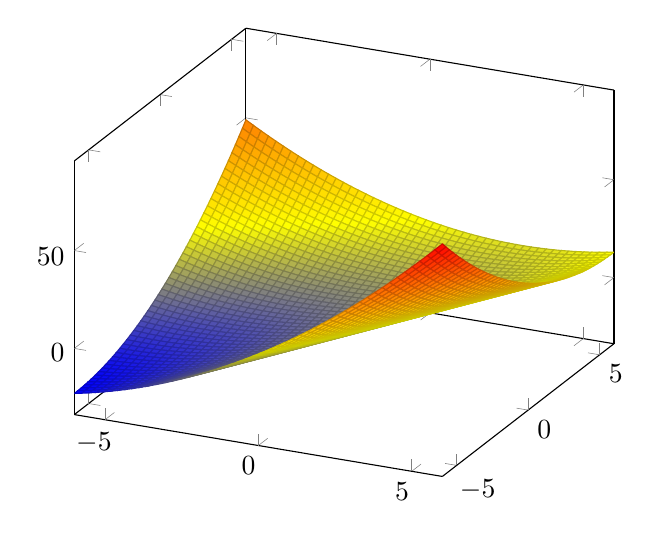
\begin{tikzpicture}
      \begin{axis}
     \addplot3[surf,domain=-6:6,samples=50]
      {0.5*(x-y)^2+3*x-5};
      \end{axis}
   \end{tikzpicture}
\end{center}


\begin{enumerate}
\item Write the function in quadratic form.
\item Does the function have any local minimum?
\end{enumerate}

